\documentclass{extbook}[14pt]
\usepackage{multicol, enumerate, enumitem, hyperref, color, soul, setspace, parskip, fancyhdr, amssymb, amsthm, amsmath, latexsym, units, mathtools}
\everymath{\displaystyle}
\usepackage[headsep=0.5cm,headheight=0cm, left=1 in,right= 1 in,top= 1 in,bottom= 1 in]{geometry}
\usepackage{dashrule}  % Package to use the command below to create lines between items
\newcommand{\litem}[1]{\item #1

\rule{\textwidth}{0.4pt}}
\pagestyle{fancy}
\lhead{}
\chead{Answer Key for Makeup Progress Quiz 3 Version B}
\rhead{}
\lfoot{1648-1753}
\cfoot{}
\rfoot{Summer C 2021}
\begin{document}
\textbf{This key should allow you to understand why you choose the option you did (beyond just getting a question right or wrong). \href{https://xronos.clas.ufl.edu/mac1105spring2020/courseDescriptionAndMisc/Exams/LearningFromResults}{More instructions on how to use this key can be found here}.}

\textbf{If you have a suggestion to make the keys better, \href{https://forms.gle/CZkbZmPbC9XALEE88}{please fill out the short survey here}.}

\textit{Note: This key is auto-generated and may contain issues and/or errors. The keys are reviewed after each exam to ensure grading is done accurately. If there are issues (like duplicate options), they are noted in the offline gradebook. The keys are a work-in-progress to give students as many resources to improve as possible.}

\rule{\textwidth}{0.4pt}

\begin{enumerate}\litem{
Determine the domain of the function below.
\[ f(x) = \frac{6}{24x^{2} +6 x -9} \]The solution is \( \text{All Real numbers except } x = -0.750 \text{ and } x = 0.500. \), which is option A.\begin{enumerate}[label=\Alph*.]
\item \( \text{All Real numbers except } x = a \text{ and } x = b, \text{ where } a \in [-2, 0.2] \text{ and } b \in [-0.3, 2.5] \)

All Real numbers except $x = -0.750$ and $x = 0.500$, which is the correct option.
\item \( \text{All Real numbers except } x = a \text{ and } x = b, \text{ where } a \in [-12.4, -11.6] \text{ and } b \in [17.4, 19.7] \)

All Real numbers except $x = -12.000$ and $x = 18.000$, which corresponds to not factoring the denominator correctly.
\item \( \text{All Real numbers.} \)

This corresponds to thinking the denominator has complex roots or that rational functions have a domain of all Real numbers.
\item \( \text{All Real numbers except } x = a, \text{ where } a \in [-2, 0.2] \)

All Real numbers except $x = -0.750$, which corresponds to removing only 1 value from the denominator.
\item \( \text{All Real numbers except } x = a, \text{ where } a \in [-12.4, -11.6] \)

All Real numbers except $x = -12.000$, which corresponds to removing a distractor value from the denominator.
\end{enumerate}

\textbf{General Comment:} Recall that dividing by zero is not a real number. Therefore the domain is all real numbers \textbf{except} those that make the denominator 0.
}
\litem{
Solve the rational equation below. Then, choose the interval(s) that the solution(s) belongs to.
\[ \frac{5}{-3x -7} + 5 = \frac{6}{9x + 21} \]The solution is \( x = -1.867 \), which is option C.\begin{enumerate}[label=\Alph*.]
\item \( x \in [2.63,2.81] \)

$x = 2.800$, which corresponds to not distributing the factor $-3x -7$ correctly when trying to eliminate the fraction.
\item \( x_1 \in [-2.06, -1.55] \text{ and } x_2 \in [1.8,3.8] \)

$x = -1.867 \text{ and } x = 2.800$, which corresponds to getting the correct solution and believing there should be a second solution to the equation.
\item \( x \in [-1.87,-0.87] \)

* $x = -1.867$, which is the correct option.
\item \( x_1 \in [-2.46, -1.99] \text{ and } x_2 \in [-1.87,0.13] \)

$x = -2.400 \text{ and } x = -1.867$, which corresponds to getting the correct solution and believing there should be a second solution to the equation.
\item \( \text{All solutions lead to invalid or complex values in the equation.} \)

This corresponds to thinking $x = -1.867$ leads to dividing by zero in the original equation, which it does not.
\end{enumerate}

\textbf{General Comment:} Distractors are different based on the number of solutions. Remember that after solving, we need to make sure our solution does not make the original equation divide by zero!
}
\litem{
Choose the equation of the function graphed below.

\begin{center}
    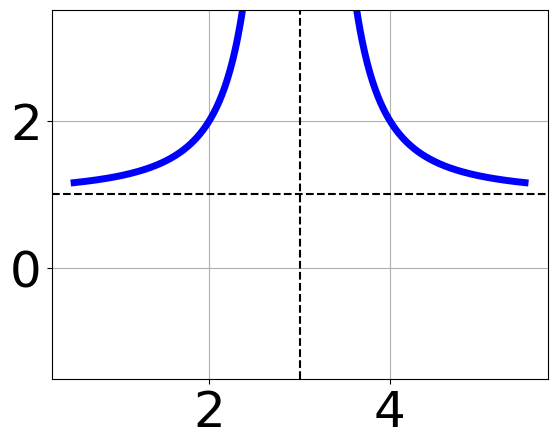
\includegraphics[width=0.5\textwidth]{../Figures/rationalGraphToEquationCopyB.png}
\end{center}


The solution is \( \text{None of the above as it should be } f(x) = \frac{-1}{x - 1} - 2 \), which is option E.\begin{enumerate}[label=\Alph*.]
\item \( f(x) = \frac{1}{(x - 1)^2} + 4 \)

Corresponds to thinking the graph was a shifted version of $\frac{1}{x^2}$, using the general form $f(x) = \frac{a}{x-h}+k$, the opposite leading coefficient, AND not noticing the $y$-value was wrong.
\item \( f(x) = \frac{1}{x - 1} + 4 \)

Corresponds to using the general form $f(x) = \frac{a}{x-h}+k$, the opposite leading coefficient AND not noticing the $y$-value was wrong.
\item \( f(x) = \frac{-1}{(x + 1)^2} + 4 \)

Corresponds to thinking the graph was a shifted version of $\frac{1}{x^2}$ not noticing the $y$-value was wrong.
\item \( f(x) = \frac{-1}{x + 1} + 4 \)

The $x$- and $y$-value of the equation does not match the graph.
\item \( \text{None of the above} \)

None of the equation options were the correct equation.
\end{enumerate}

\textbf{General Comment:} Remember that the general form of a basic rational equation is $ f(x) = \frac{a}{(x-h)^n} + k$, where $a$ is the leading coefficient (and in this case, we assume is either $1$ or $-1$), $n$ is the degree (in this case, either $1$ or $2$), and $(h, k)$ is the intersection of the asymptotes.
}
\litem{
Choose the graph of the equation below.
\[ f(x) = \frac{1}{x + 3} - 1 \]The solution is the graph below, which is option A.
    \begin{center}
        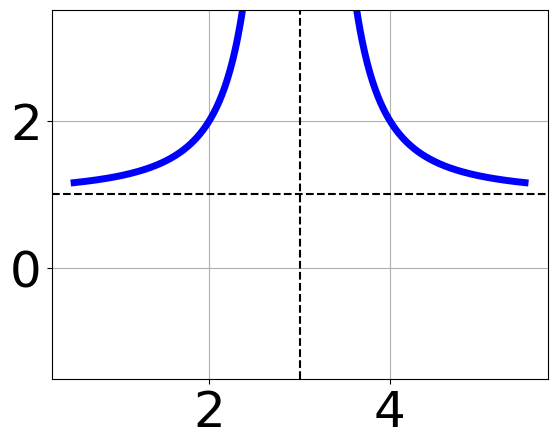
\includegraphics[width=0.3\textwidth]{../Figures/rationalEquationToGraphCopyAB.png}
    \end{center}\begin{enumerate}[label=\Alph*.]
\begin{multicols}{2}
\item 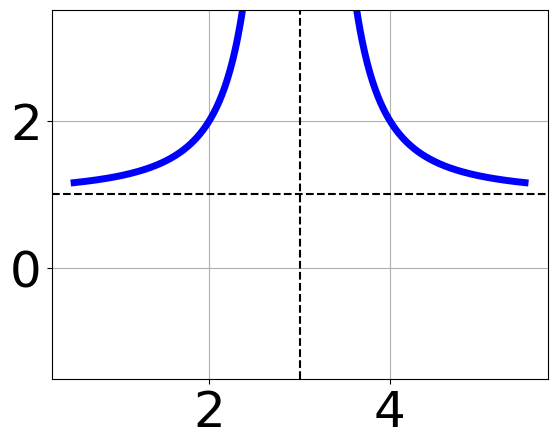
\includegraphics[width = 0.3\textwidth]{../Figures/rationalEquationToGraphCopyAB.png}
\item 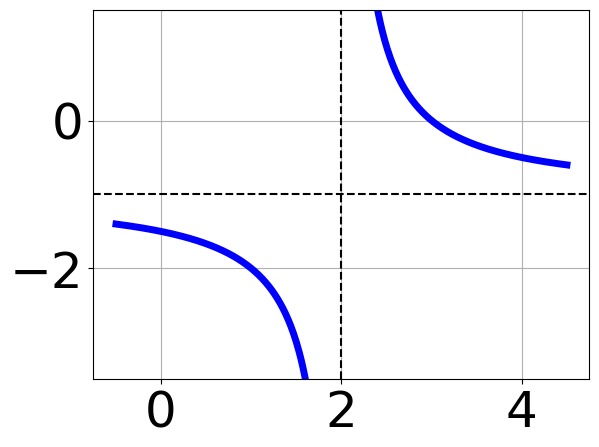
\includegraphics[width = 0.3\textwidth]{../Figures/rationalEquationToGraphCopyBB.png}
\item 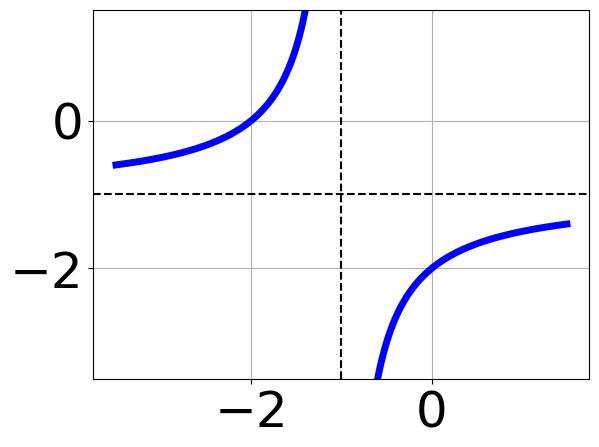
\includegraphics[width = 0.3\textwidth]{../Figures/rationalEquationToGraphCopyCB.png}
\item 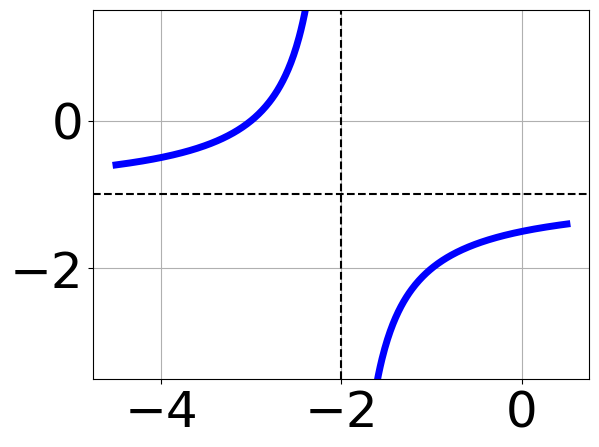
\includegraphics[width = 0.3\textwidth]{../Figures/rationalEquationToGraphCopyDB.png}
\end{multicols}\item None of the above.\end{enumerate}
\textbf{General Comment:} Remember that the general form of a basic rational equation is $ f(x) = \frac{a}{(x-h)^n} + k$, where $a$ is the leading coefficient (and in this case, we assume is either $1$ or $-1$), $n$ is the degree (in this case, either $1$ or $2$), and $(h, k)$ is the intersection of the asymptotes.
}
\litem{
Determine the domain of the function below.
\[ f(x) = \frac{3}{12x^{2} -36 x + 24} \]The solution is \( \text{All Real numbers except } x = 1.000 \text{ and } x = 2.000. \), which is option D.\begin{enumerate}[label=\Alph*.]
\item \( \text{All Real numbers except } x = a \text{ and } x = b, \text{ where } a \in [14.7, 16.9] \text{ and } b \in [17, 18.2] \)

All Real numbers except $x = 16.000$ and $x = 18.000$, which corresponds to not factoring the denominator correctly.
\item \( \text{All Real numbers except } x = a, \text{ where } a \in [-1.1, 1.7] \)

All Real numbers except $x = 1.000$, which corresponds to removing only 1 value from the denominator.
\item \( \text{All Real numbers except } x = a, \text{ where } a \in [14.7, 16.9] \)

All Real numbers except $x = 16.000$, which corresponds to removing a distractor value from the denominator.
\item \( \text{All Real numbers except } x = a \text{ and } x = b, \text{ where } a \in [-1.1, 1.7] \text{ and } b \in [1.7, 2.9] \)

All Real numbers except $x = 1.000$ and $x = 2.000$, which is the correct option.
\item \( \text{All Real numbers.} \)

This corresponds to thinking the denominator has complex roots or that rational functions have a domain of all Real numbers.
\end{enumerate}

\textbf{General Comment:} Recall that dividing by zero is not a real number. Therefore the domain is all real numbers \textbf{except} those that make the denominator 0.
}
\litem{
Solve the rational equation below. Then, choose the interval(s) that the solution(s) belongs to.
\[ \frac{3}{5x + 4} + -7 = \frac{2}{-20x -16} \]The solution is \( x = -0.700 \), which is option B.\begin{enumerate}[label=\Alph*.]
\item \( x \in [0.87,0.94] \)

$x = 0.900$, which corresponds to not distributing the factor $5x + 4$ correctly when trying to eliminate the fraction.
\item \( x \in [-1.7,1.3] \)

* $x = -0.700$, which is the correct option.
\item \( \text{All solutions lead to invalid or complex values in the equation.} \)

This corresponds to thinking $x = -0.700$ leads to dividing by zero in the original equation, which it does not.
\item \( x_1 \in [-0.7, -0.69] \text{ and } x_2 \in [0.9,5.9] \)

$x = -0.700 \text{ and } x = 0.900$, which corresponds to getting the correct solution and believing there should be a second solution to the equation.
\item \( x_1 \in [-0.79, -0.72] \text{ and } x_2 \in [-0.7,0.3] \)

$x = -0.771 \text{ and } x = -0.700$, which corresponds to getting the correct solution and believing there should be a second solution to the equation.
\end{enumerate}

\textbf{General Comment:} Distractors are different based on the number of solutions. Remember that after solving, we need to make sure our solution does not make the original equation divide by zero!
}
\litem{
Choose the graph of the equation below.
\[ f(x) = \frac{-1}{x - 2} - 2 \]The solution is the graph below, which is option B.
    \begin{center}
        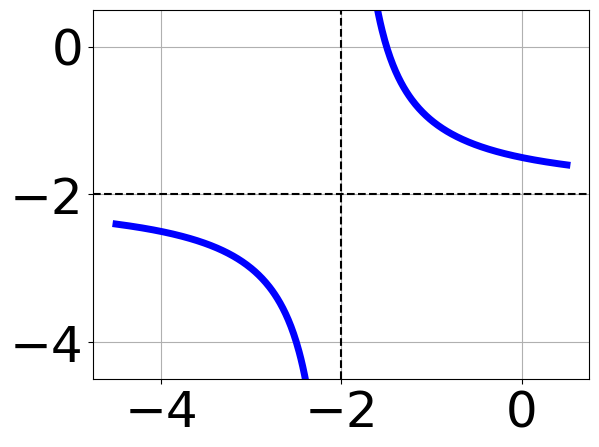
\includegraphics[width=0.3\textwidth]{../Figures/rationalEquationToGraphBB.png}
    \end{center}\begin{enumerate}[label=\Alph*.]
\begin{multicols}{2}
\item 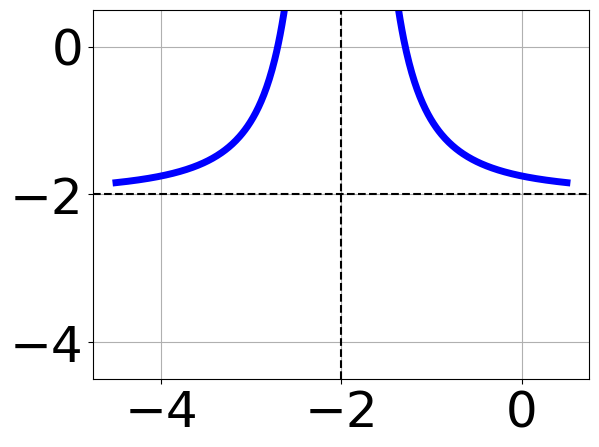
\includegraphics[width = 0.3\textwidth]{../Figures/rationalEquationToGraphAB.png}
\item 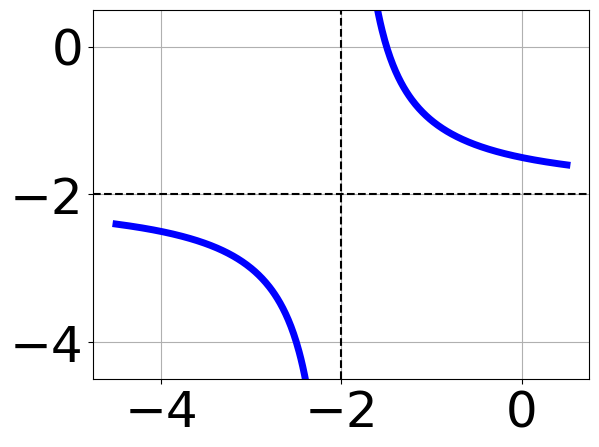
\includegraphics[width = 0.3\textwidth]{../Figures/rationalEquationToGraphBB.png}
\item 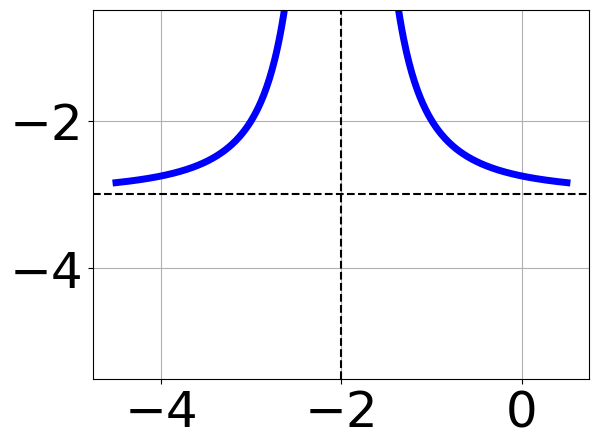
\includegraphics[width = 0.3\textwidth]{../Figures/rationalEquationToGraphCB.png}
\item 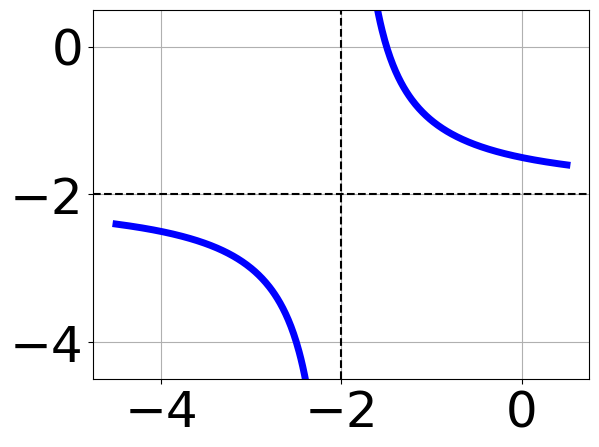
\includegraphics[width = 0.3\textwidth]{../Figures/rationalEquationToGraphDB.png}
\end{multicols}\item None of the above.\end{enumerate}
\textbf{General Comment:} Remember that the general form of a basic rational equation is $ f(x) = \frac{a}{(x-h)^n} + k$, where $a$ is the leading coefficient (and in this case, we assume is either $1$ or $-1$), $n$ is the degree (in this case, either $1$ or $2$), and $(h, k)$ is the intersection of the asymptotes.
}
\litem{
Choose the equation of the function graphed below.

\begin{center}
    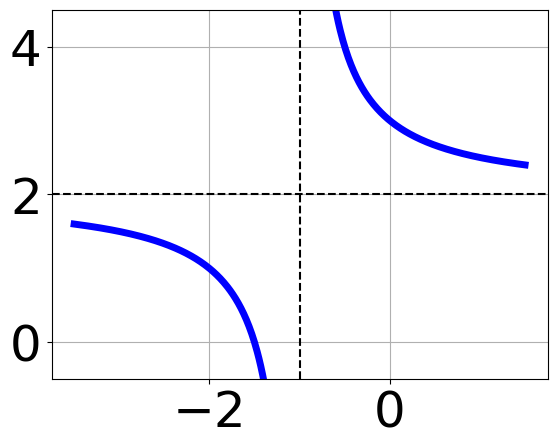
\includegraphics[width=0.5\textwidth]{../Figures/rationalGraphToEquationB.png}
\end{center}


The solution is \( f(x) = \frac{1}{x + 1} + 2 \), which is option C.\begin{enumerate}[label=\Alph*.]
\item \( f(x) = \frac{-1}{(x - 1)^2} + 2 \)

Corresponds to thinking the graph was a shifted version of $\frac{1}{x^2}$, using the general form $f(x) = \frac{a}{x+h}+k$, and the opposite leading coefficient.
\item \( f(x) = \frac{-1}{x - 1} + 2 \)

Corresponds to using the general form $f(x) = \frac{a}{x+h}+k$ and the opposite leading coefficient.
\item \( f(x) = \frac{1}{x + 1} + 2 \)

This is the correct option.
\item \( f(x) = \frac{1}{(x + 1)^2} + 2 \)

Corresponds to thinking the graph was a shifted version of $\frac{1}{x^2}$.
\item \( \text{None of the above} \)

This corresponds to believing the vertex of the graph was not correct.
\end{enumerate}

\textbf{General Comment:} Remember that the general form of a basic rational equation is $ f(x) = \frac{a}{(x-h)^n} + k$, where $a$ is the leading coefficient (and in this case, we assume is either $1$ or $-1$), $n$ is the degree (in this case, either $1$ or $2$), and $(h, k)$ is the intersection of the asymptotes.
}
\litem{
Solve the rational equation below. Then, choose the interval(s) that the solution(s) belongs to.
\[ \frac{5x}{3x + 5} + \frac{-2x^{2}}{18x^{2} +39 x + 15} = \frac{-6}{6x + 3} \]The solution is \( \text{All solutions are invalid or lead to complex values in the equation.} \), which is option D.\begin{enumerate}[label=\Alph*.]
\item \( x_1 \in [-2.39, -1.64] \text{ and } x_2 \in [-0.56,-0.38] \)

$x = -1.667 \text{ and } x = -0.500$, which corresponds to solving $3x + 5 = 0$ and $6x + 3 = 0$ and treating them as solutions to the equation.
\item \( x \in [-2.39,-1.64] \)

$x = -1.667$, which corresponds to solving $3x + 5 = 0$ and treating it as a solution to the equation.
\item \( x_1 \in [-1.48, -0.61] \text{ and } x_2 \in [-0.17,1.79] \)

$x = -1.335 \text{ and } x = 0.304$, which corresponds to making the discriminant from the Quadratic Formula positive to avoid complex solutions.
\item \( \text{All solutions lead to invalid or complex values in the equation.} \)

* The equation leads to solving $32x^{2} +33 x + 30=0$, which leads to complex solutions. This is the correct option.
\item \( x \in [-0.75,-0.03] \)

$x = -0.500$, which corresponds to solving $6x + 3 = 0$ and treating it as a solution to the equation.
\end{enumerate}

\textbf{General Comment:} Distractors are different based on the number of solutions. Remember that after solving, we need to make sure our solution does not make the original equation divide by zero!
}
\litem{
Solve the rational equation below. Then, choose the interval(s) that the solution(s) belongs to.
\[ \frac{-5x}{2x -6} + \frac{-6x^{2}}{14x^{2} -28 x -42} = \frac{2}{7x + 7} \]The solution is \( \text{There are two solutions: } x = 0.245 \text{ and } x = -1.196 \), which is option D.\begin{enumerate}[label=\Alph*.]
\item \( \text{All solutions lead to invalid or complex values in the equation.} \)


\item \( x_1 \in [0.16, 0.32] \text{ and } x_2 \in [2,6] \)


\item \( x \in [-1.05,-0.78] \)


\item \( x_1 \in [0.16, 0.32] \text{ and } x_2 \in [-6.2,2.8] \)

* $x = 0.245 \text{ and } x = -1.196$, which is the correct option.
\item \( x \in [-1.23,-1.17] \)


\end{enumerate}

\textbf{General Comment:} Distractors are different based on the number of solutions. Remember that after solving, we need to make sure our solution does not make the original equation divide by zero!
}
\end{enumerate}

\end{document}